\begin{frame}{Subsistema de izaje}
  \begin{block}{Características del sistema}
    Controla la elevación de la carga mediante:
    \begin{itemize}
      \item Motor eléctrico accionando un \textbf{tambor}
      \item Sistema de cableado con relación de transmisión \textbf{2:1} (aparejo móvil)
      \item Carga suspendida: \textbf{2 grados de libertad}
    \end{itemize}
    Característica clave:
    \begin{itemize}
    \item\alert{Dinámica híbrida}
    \end{itemize}
  \end{block}
\end{frame}

\begin{frame}{Parámetros discretos}
  \begin{block}{Masa total ($m_l$)}
    \[
    m_l(\text{TLK}) = 
    \begin{cases} 
      M_s & \text{si TLK} = 0 \text{ (solo spreader)} \\[6pt]
      M_s + M_{cX} & \text{si TLK} = 1 \text{ (spreader + contenedor)}
    \end{cases}
    \]
  \end{block}

  \begin{block}{Altura de la carga ($h_c$)}
    \[
    h_c(\text{TLK}) = 
    \begin{cases} 
      0 & \text{si TLK} = 0 \\
      H_c & \text{si TLK} = 1
    \end{cases}
    \]
  \end{block}
\end{frame}

\begin{frame}{Ecuaciones de movimiento de la carga}
  \begin{block}{Dinámicas acopladas}
    \begin{equation*}
      m_l(\textcolor{signalcolor}{TLK}) \, \frac{d \, v_{lx}(t)}{dt} = -2 F_{hw}(t,l(t)-l_h(t)) \, \sin\theta_l(t) + F_{cx}(t, \delta y)
    \end{equation*}
    \begin{equation*}
        m_l(\textcolor{signalcolor}{TLK}) \, \frac{d \, v_{ly}(t)}{dt} = 2 F_{hw}(t,l(t)-l_h(t)) \, \cos\theta_l(t) - m_l(\textcolor{signalcolor}{TLK}) \, g + F_{cy}(t, \delta y)
    \end{equation*}
    \begin{equation*}
      \delta y = y_l(t) - h_c(\textcolor{signalcolor}{TLK}) - y_{c0}(x_l(t), t)
    \end{equation*}
  \end{block}
\end{frame}

\begin{frame}{Interacción con el entorno}
  \begin{block}{Condición de contacto}
    Cuando: $\delta y \le 0$ 
  \end{block}

  \begin{block}{Fuerza vertical}
    \[
    F_{cy} = 
    \begin{cases} 
      K_{cy}(y_{c0} - (y_l - h_c)) - b_{cy} v_{ly} & \text{(Apoyado)} \\[4pt]
      0 & \text{(Suspendido)}
    \end{cases}
    \]
  \end{block}

  \begin{block}{Fuerza horizontal}
    \[
    F_{cx} = 
    \begin{cases} 
      -b_{cx} v_{lx} & \text{(Apoyado)} \\[4pt]
      0 & \text{(Suspendido)}
    \end{cases}
    \]
  \end{block}
\end{frame}

\begin{frame}{Acoplamiento elástico del cable}
  \begin{block}{Resorte-amortiguador con rigidez variable}
    La rigidez y amortiguamiento escalan con la longitud del cable bajo tensión:
    \[
    K_{hw}(l_h) = \frac{k_{hwu}}{2 l_h + L_{h0}} \quad ; \quad b_{hw}(l_h) = b_{hwu}(2 l_h + L_{h0})
    \]
  \end{block}

  \begin{block}{Fuerza de tensión}
    \[
    F_{hw} = 
    \begin{cases} 
      K_{hw}(l_h) \cdot 2(l - l_h) + b_{hw}(l_h) \cdot 2(\dot{l} - \dot{l}_h) & \text{(Tenso)} \\[4pt]
      0 & \text{(Flojo)}
    \end{cases}
    \]
  \end{block}
\end{frame}

\begin{frame}{Dinámica del accionamiento}
  \small
  \begin{block}{Ecuaciones de  los dos ejes}
    \begin{itemize}
      \item \textbf{Eje lento(tambor):}
      \begin{equation*}
        J_{hd+hEb} \, \frac{d \, \omega_{hd}(t)}{dt} = T_{hd}(t) + T_{hEb}(t,\textcolor{signalcolor}{BRK_{hE}}) - b_{hd} \, \omega_{hd}(t) - T_{hdl}(t)
      \end{equation*}
      \item \textbf{Eje rápido(motor):} 
      \begin{equation*}
        J_{hm+hb} \, \frac{d \, \omega_{hm}(t)}{dt} = T_{hm}(t) + T_{hb}(t,\textcolor{signalcolor}{BRK_{h}}) - b_{hm} \, \omega_{hm}(t) - T_{hml}(t)
      \end{equation*}
    \end{itemize}
  \end{block}

  \vspace{0.2cm}
  \begin{block}{Relación cinemática}
    \[
    v_h(t) = \frac{r_{hd} \omega_{hd}(t)}{2} = -\frac{dl_h}{dt}
    \]
    Factor 2 divide la velocidad tangencial del tambor
  \end{block}
\end{frame}

\begin{frame}{Frenos mecánicos}
\begin{figure}
  \centering
  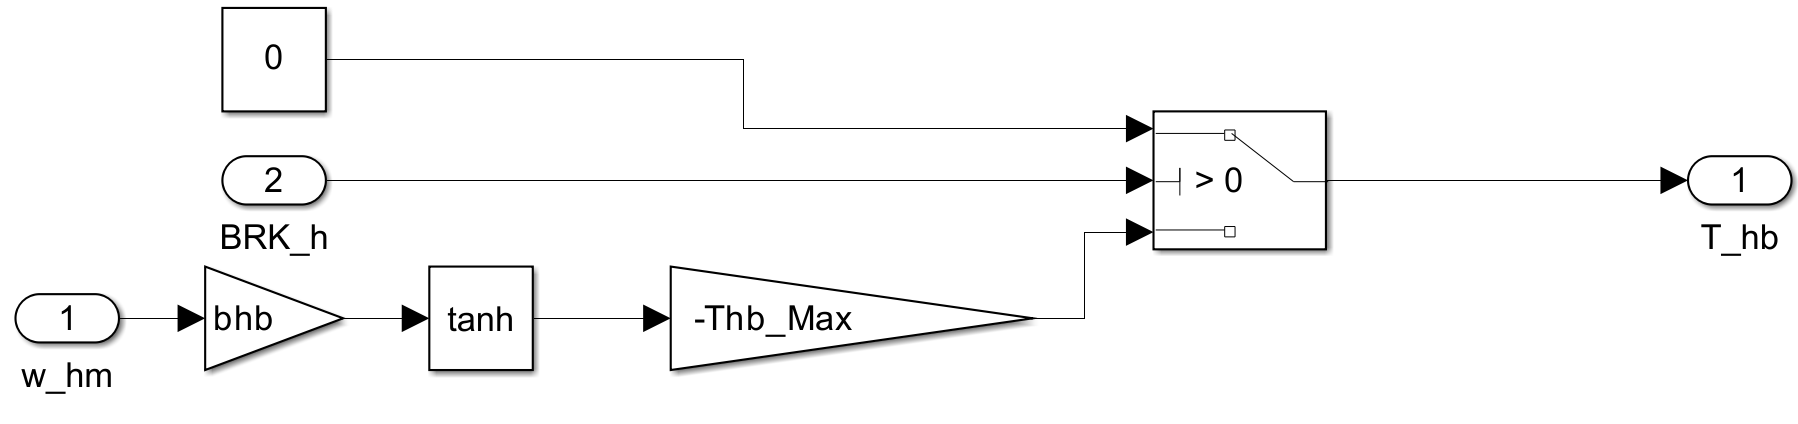
\includegraphics[width=0.8\textwidth]{freno_izaje.png}
  \caption{Freno mecánico de operación izaje}
\end{figure}
\begin{figure}
  \centering
  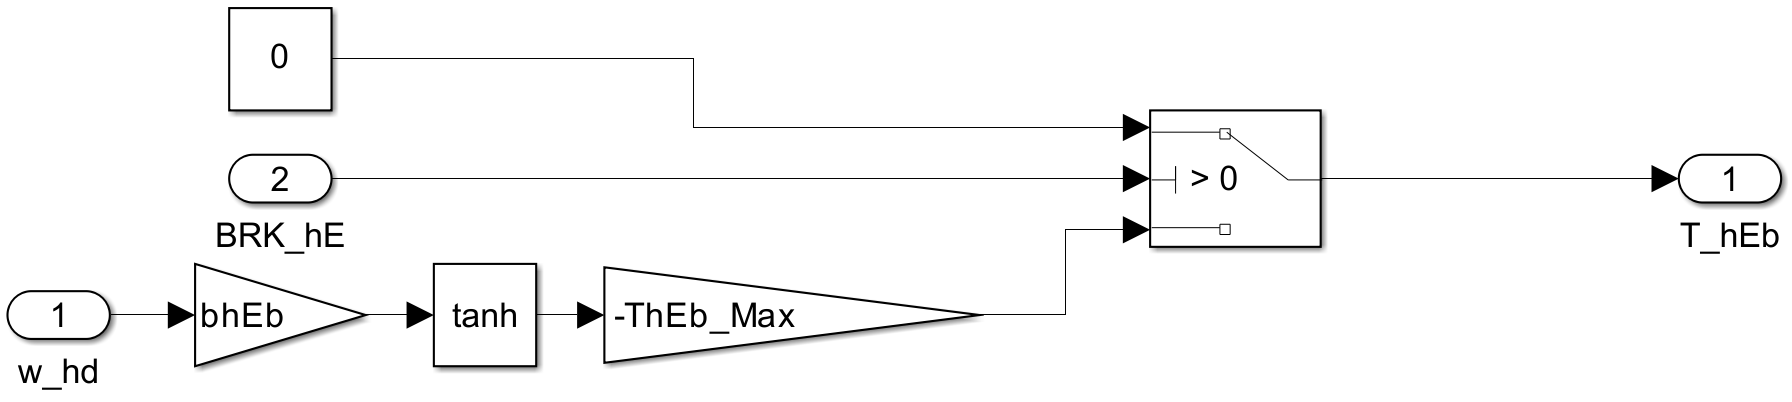
\includegraphics[width=0.8\textwidth]{freno_izaje_e.png}
  \caption{Freno mecánico de emergencia izaje}
\end{figure}
\end{frame}

\begin{frame}{Modelo equivalente referido al motor}
  \begin{block}{Reducción eje equivalente}
    Al igual que el carro, se refiere la dinámica del tambor al motor usando $i_h$:
  \end{block}

  \vspace{-0.2cm}
  \[
  J_{h,eq} = J_{hm+hb} + \frac{J_{hd+hEb}}{i_h^2}
  \]

  \vspace{-0.3cm}
  \[
  b_{h,eq} = b_{hm} + \frac{b_{hd}}{i_h^2} 
  \]
  \begin{block}{Variables auxiliares}
    \vspace{-0.2cm}
    \begin{itemize}
      \item Longitud geométrica: $l(t) = \sqrt{(x_l - x_t)^2 + (Y_{t0} - y_l)^2}$
      \item Velocidad de cambio: $\frac{dl}{dt} = \frac{(x_l - x_t)(v_{lx} - v_t) - (Y_{t0} - y_l)v_{ly}}{l}$
      \item Ángulo de balanceo: $\theta_l = \text{atan2}\left(\frac{x_l - x_t}{Y_{t0} - y_l}\right)$
    \end{itemize}
  \end{block}
\end{frame}

\begin{frame}{Subsistema izaje completo}
\begin{figure}
  \centering
  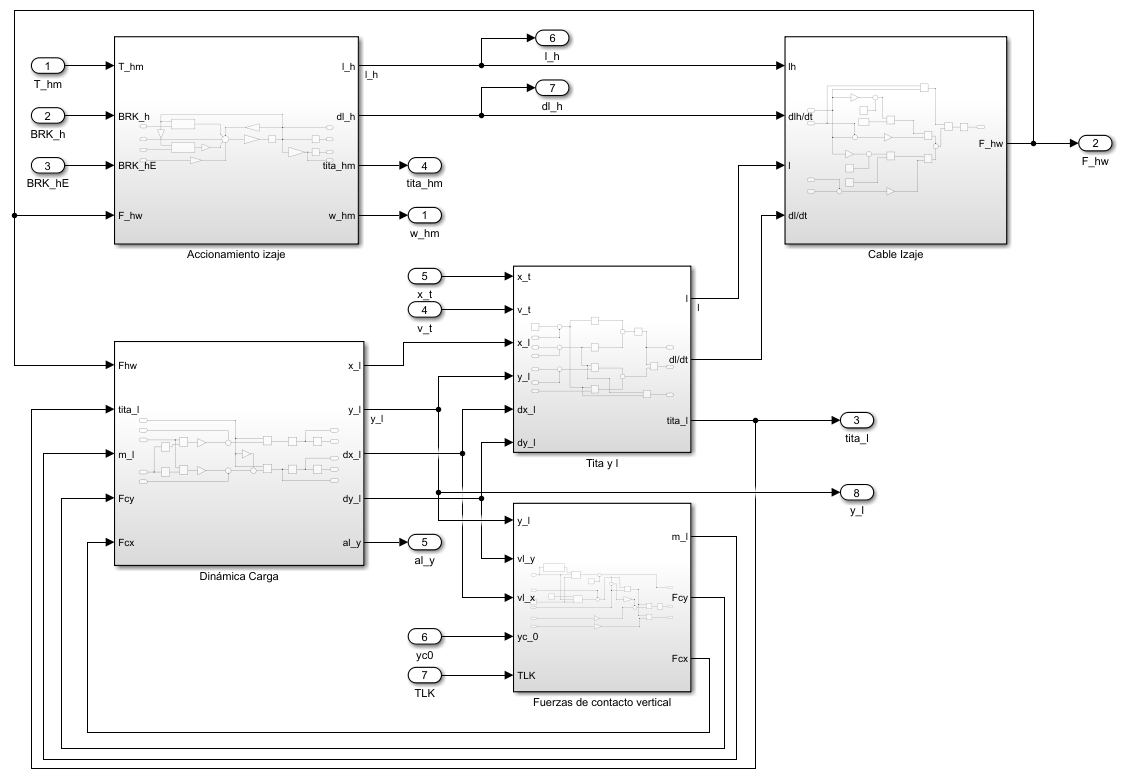
\includegraphics[width=0.77\textwidth]{modelo_izaje.png}
  %\caption{Diagrama de bloques del subsistema de izaje}
\end{figure}
  
\end{frame}

\begin{frame}{Sensores}
  \begin{block}{Sensor carro}
    \begin{itemize}
    \item \textbf{Encoder:} Mide la posición angular del motor del carro $\theta_{tm}(t)$
    \[
  x_t(t) = \theta_{tm}(t) \, \frac{r_{tm}}{i_t}
    \]
    \end{itemize}
  \end{block}
  \begin{block}{Sensores izaje}
    \begin{itemize}
    \item \textbf{Encoder:} Mide posición angular del motor de izaje $\theta_{hm}(t)$
    \[
    y_h(t) = \theta_{hm}(t) \, \frac{r_{hd}}{2\,i_h}
    \]
    \item \textbf{Celda de carga:} Mide fuerza de tensión $F_{hw}(t)$ en el cable de izaje
    \item \textbf{Sensor de ángulo de spreader:} Mide ángulo de balanceo $\theta_l(t)$ y velocidad angular $\dot{\theta}_l(t)$ 
    de la carga suspendida
    \end{itemize}
  \end{block}
\end{frame}

\begin{frame}{Fines de carrera}
  \begin{block}{FC del carro}
    \vspace{0.2cm}
    \begin{columns}[T]
      \begin{column}{0.5\textwidth}
        \[
        \text{FC}_{t,\text{der}} = 
        \begin{cases} 
          0 & \text{si } x_t < x_{t\max} \\[4pt]
          1 & \text{si } x_t \ge x_{t\max} \\[4pt]
          1 & \text{si } x_t \ge x_{t\max} + 0.5 \text{ m (E)}
        \end{cases}
        \]
      \end{column}
      \begin{column}{0.5\textwidth}
        \[
        \text{FC}_{t,\text{izq}} = 
        \begin{cases} 
          0 & \text{si } x_t > x_{t\min} \\
          1 & \text{si } x_t \le x_{t\min} \\[4pt]
          1 & \text{si } x_t \le x_{t\min} + 0.5 \text{ m (E)}
        \end{cases}
        \]
      \end{column}
    \end{columns}
  \end{block}
    \begin{block}{FC del izaje}
    \vspace{0.2cm}
    \begin{columns}[T]
      \begin{column}{0.5\textwidth}
        \[
        \text{FC}_{h,\text{sup}} = 
        \begin{cases} 
          0 & \text{si } y_h < y_{h\max} \\[4pt]
          1 & \text{si } y_h \ge y_{h\max} \\[4pt]
          1 & \text{si } y_h \ge y_{h\max} + 0.5 \text{ m (E)}
        \end{cases}
        \]
      \end{column}
      \begin{column}{0.5\textwidth}
        \[
        \text{FC}_{h,\text{inf}} = 
        \begin{cases} 
          0 & \text{si } y_h > y_{h\min} \\[4pt]
          1 & \text{si } y_h \le y_{h\min}  \\[4pt]
          1 & \text{si } y_h \le y_{h\min} + 0.5 \text{ m (E)}
        \end{cases}
        \]
      \end{column}
    \end{columns}
  \end{block}
\end{frame}



\begin{frame}{Modelo sensores}
  \begin{columns}[T]
    \begin{column}{0.48\textwidth}
      \vspace{1cm}
      \centering
      \begin{figure}
      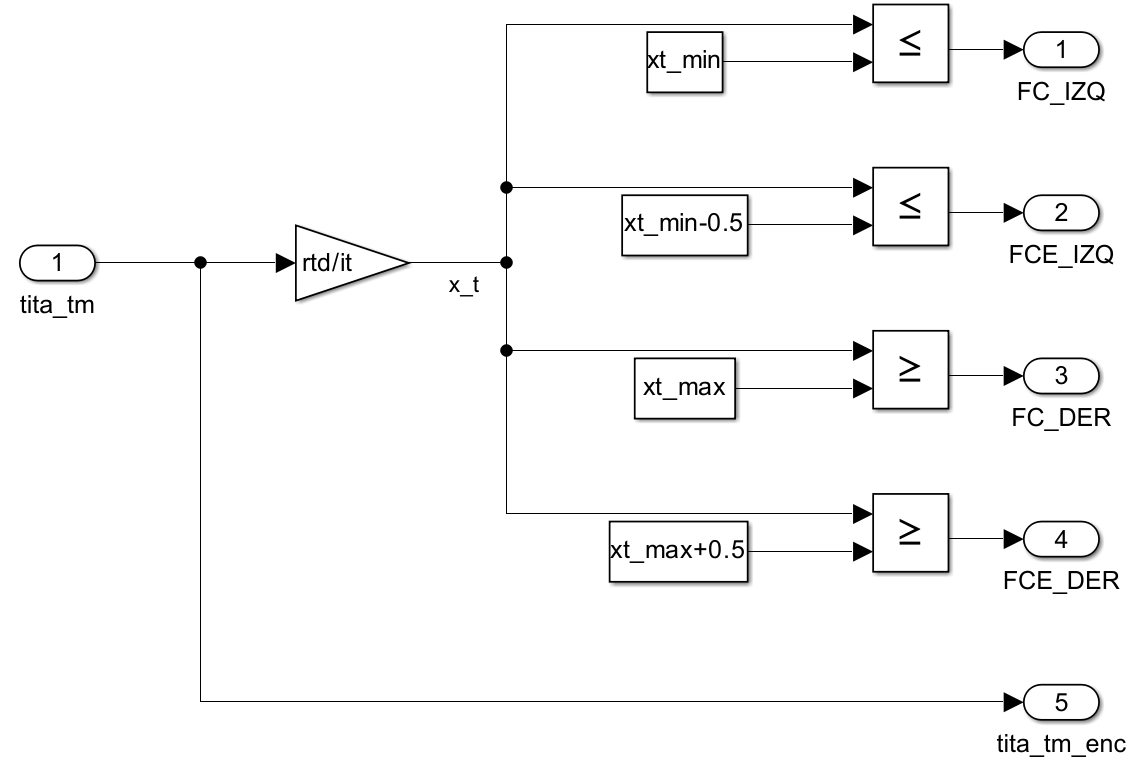
\includegraphics[width=\textwidth]{sensores_carro.png}
      \caption{Diagrama de bloques sensores carro e izaje Simulink}
      \end{figure}
    \end{column}
    \begin{column}{0.48\textwidth}
      \centering
      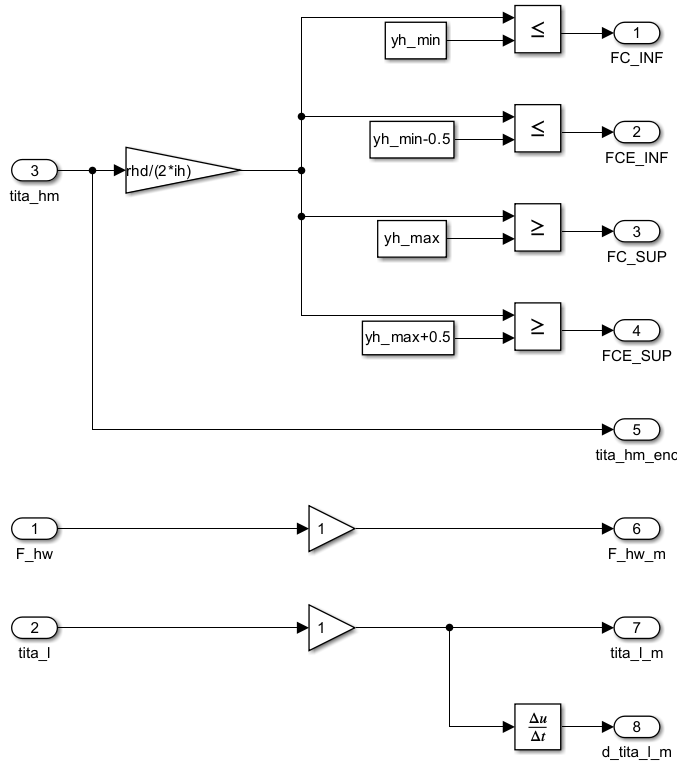
\includegraphics[width=\textwidth]{sensores_izaje.png}
    \end{column}
  \end{columns}
\end{frame}


\begin{frame}{Moduladores de torque}
  \begin{block}{Función en la simulación}
    Modelan las limitaciones de los \textbf{accionamientos reales} (motores eléctricos)
    \begin{itemize}
      \item No es posible aplicar torque instantáneo como una fuerza mecánica ideal
      \item Los motores reales tienen capacidad limitada y retardo dinámico
    \end{itemize}
  \end{block}

  \begin{block}{Dos funciones clave}
    \begin{enumerate}
      \item \textbf{Saturación}: limita torque a máximo permitido $T_{\max}$
      \item \textbf{Filtrado}: modela retardo electromagnético con constante $\tau = 1$ ms
    \end{enumerate}
  \end{block}
  \begin{block}{Ecuación diferencial}
    Vincula el torque limitado comandado $T_{\text{Lim}}^*(t)$ con el torque físico real $T(t)$:
    \vspace{-0.2cm}
    \[
    \tau \frac{dT(t)}{dt} = T_{\text{Lim}}^*(t) - T(t)
    \]
  \end{block}

\end{frame}


\begin{frame}{Modulador del carro}
  \begin{block}{Ecuación}
    \[
T_{tm\ Lim}^*(k \, T_{s2} \leq t < (k+1) \, T_{s2}) = \text{min}\left(+T_{tm\max}, \text{max}\left(-T_{tm\max}, T_{tm}^*(k \, T_{s2})\right)\right)
    \]
  \end{block}
  \begin{figure}
  \centering
  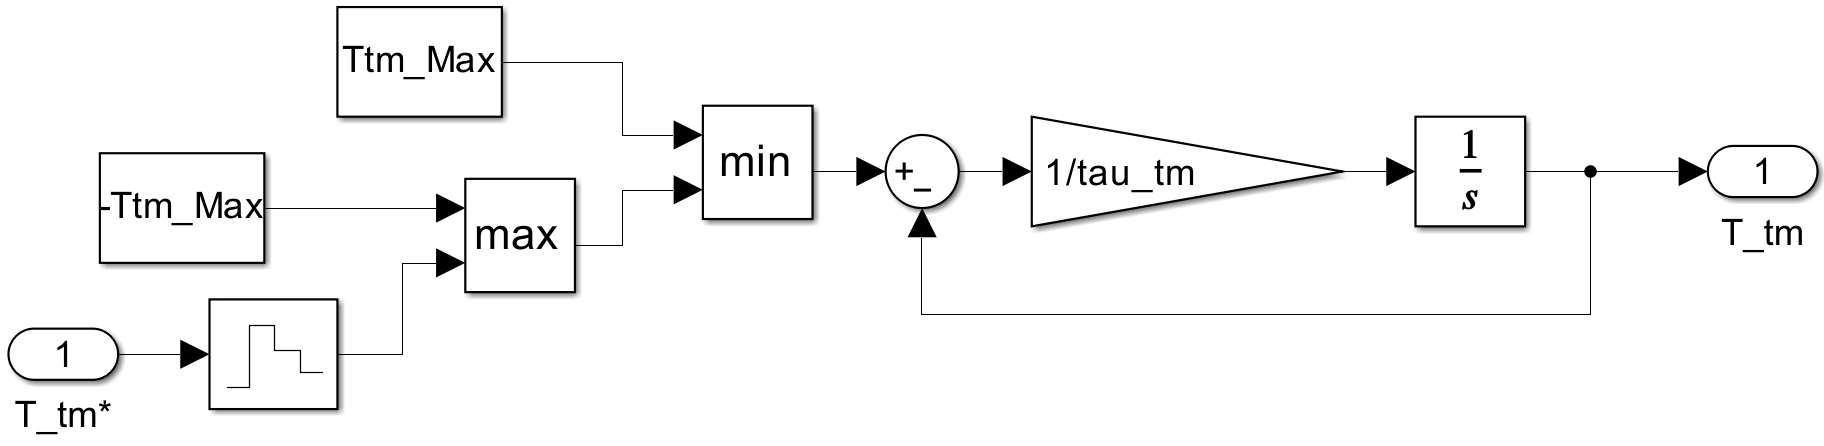
\includegraphics[width=1\textwidth]{modulador_carro.png}
  \caption{Diagrama de bloques del modulador de torque del carro}
  \end{figure}
\end{frame}

